\documentclass[12pt]{article}

\usepackage{fullpage}
%\usepackage[dvips]{graphics}
%\usepackage{amssymb}
%\usepackage{amsmath}
\usepackage{amsthm}
\usepackage{appendix}
%\renewcommand{\baselinestretch}{2}
\usepackage{setspace}
\doublespacing

\textheight 9.0in
\leftmargin 1.0in
%\rightmargin 1.0in

\usepackage{latexsym,epsfig,graphicx,amsmath,amssymb,amscd,multirow,chicago,psfrag}
\def\bbeta{\mbox{\boldmath$\beta$}}
\def\btheta{\mbox{\boldmath$\theta$}}
\def\bSigma{\mbox{\boldmath$\Sigma$}}
\def\bTheta{\mbox{\boldmath$\Theta$}}
\def\bOmega{\mbox{\boldmath$\Omega$}}
\def\bdelta{\mbox{\boldmath$\delta$}}
\def\bgamma{\mbox{\boldmath$C$}}
\def\bsigma{\mbox{\boldmath$\sigma$}}
\def\blambda{\mbox{\boldmath$\lambda$}}
\def\bomega{\mbox{\boldmath$\omega$}}
\def\brho{\mbox{\boldmath$\rho$}}
\def\btau{\mbox{\boldmath$\tau$}}
\def\bnu{\mbox{\boldmath$\nu$}}
\def\bxi{\mbox{\boldmath$\xi$}}
\newcommand{\mb}[1]{\mbox{\boldmath$#1$}}
\newcommand{\cov}{\text{cov}}
\newcommand{\mbzero}{\mathbf{0}}
\newcommand{\mbX}{\mathbf{X}}
\newtheorem{theorem}{Theorem}
\newtheorem{lemma}[theorem]{Lemma}
\newtheorem{property}{Property}

\begin{document}
%%%%%%%%%%%%%%%%%%%%%%%%%%%%%%%%%%%%%%%%%%%%%%%%%%%%%%%%%%%%%%%%%%%%%%%%%%%%%%%%%%%%%%%%%%%%%%%%%%%%%%%%%%%%%%%%%
\title{Supplementary Materials to ``Model-Based Sampling Design for Multivariate Geostatistics''}
\author{Jie Li\thanks{Jie Li (Email: jieli@vt.edu) is Research Assistant Professor, Department of Statistics, Virginia Polytechnic Institute and State University, Blacksburg, VA 24601.} \ \ and \ \ Dale L. Zimmerman\thanks{Dale L. Zimmerman (Email: dale-zimmerman@uiowa.edu) is Robert V.\ Hogg Professor, Department of Statistics and
Actuarial Science, 241 Schaeffer Hall, University of Iowa, Iowa City, IA 52242.}}

\date{}
%%%%%%%%%%%%%%%%%%%%%%%%%%%%%%%%%%%%%%%%%%%%%%%%%%%%%%%%%%%%%%%%%%%%%%%%%%%%%%%%%%%%%%%%%%%%%%%%%%%%%%%%%%%%%%%%%
\maketitle

\begin{abstract}
These supplementary materials provide supplemental tables and figures referenced in the paper, a description of the simulated annealing algorithm used to search for optimal designs in the large examples, and proofs of Theorems 1 and 2.
\end{abstract}

%%%%%%%%%%%%%%%%%%%%%%%%%%%%%%%%%%%%%%%%%%%%%%%%%%%%%%%%%%%%%%%%%%%%%%%%%%%%%%%%%%%%%%%%%%%%%%%%%%%%%%%%%%%%%%%%%
%\newpage
\renewcommand{\baselinestretch}{1.5}
%section 7.3.1
%\noindent \Large\textbf{Appendix A: Simulated Annealing
    %Algorithm}\label{sec:saa}

\newpage
\section{Supplemental Tables}
\vspace{5mm}
\renewcommand{\baselinestretch}{1.0}
%section 7.3.1
\noindent
Supplemental Table 1:  Relative MPEV-efficiencies of locally MPEV-optimal designs ($[\gamma_{MPEV}$\\$(D^{*}_{MPEV}(\btheta);\btheta)/\gamma_{MPEV}(D^{*}_{MPEV}(\btheta^{\prime});\btheta)]\times 100\%$, with $\btheta$ corresponding to rows and $\btheta^{\prime}$ to columns) and the locally worst design ($[\gamma_{MPEV}(D^{*}_{MPEV}(\btheta);\btheta)/\max_{D}\gamma_{MPEV}(D;\btheta)]\times 100\%$), for nine cases of cross-correlation and spatial correlation parameters in the Mat(0.5) examples.
%If we use $D^{*}_{MPEV_{row_{i}}}$ and $D^{*}_{MPEV_{col_{j}}}$ to denote the locally optimal design corresponds to the $i$th row and $j$th column, respectively, then the $(i,j)$th element in the table is $[\gamma_{MPEV}(D^{*}_{MPEV_{row_{i}}}(\btheta);\btheta)/\gamma_{MPEV}(D^{*}_{MPEV_{col_{j}}};\btheta) ]\times 100\%$.
{\footnotesize
\vspace{.05in}
\begin{center}
\begin{tabular}{|cc|rrrrrrrrrr|}
\hline
&& \multicolumn{10}{c|}{Toy example}  \\
%$(\rho_c,\rho)$ & (0.2,0.2) & (0.2,0.5) & (0.2,0.8) & (0.5,0.2) & (0.5,0.5) & (0.5,0.8) & (0.8,0.2) & (0.8,0.5) & (0.8,0.8) & (f) \\
           & $\rho_{c}$ &  0.2 & 0.2 & 0.2 & 0.5 & 0.5 & 0.5 & 0.8 & 0.8 & 0.8 & locally worst \\
$\rho_{c}$ & $\rho$     &  0.2 & 0.5 & 0.8 & 0.2 & 0.5 & 0.8 & 0.2 & 0.5 & 0.8 & design \\
\hline
0.2 & 0.2 & 100 & 98  & 98  & 99  & 100 & 98  & 99  & 99  & 95  & 65  \\
0.2 & 0.5 & 99  & 100 & 100 & 89  & 97  & 100 & 89  & 89  & 93  & 28  \\
0.2 & 0.8 & 92  & 100 & 100 & 75  & 89  & 100 & 75  & 75  & 85  & 10  \\
0.5 & 0.2 & 93  & 91  & 91  & 100 & 99  & 91  & 100 & 100 & 95  & 60  \\
0.5 & 0.5 & 99  & 99  & 99  & 95  & 100 & 99  & 95  & 95  & 97  & 30  \\
0.5 & 0.8 & 92  & 100 & 100 & 81  & 91  & 100 & 81  & 81  & 90  & 11  \\
0.8 & 0.2 & 66  & 64  & 64  & 100 & 92  & 64  & 100 & 100 & 91  & 38  \\
0.8 & 0.5 & 77  & 75  & 75  & 100 & 91  & 75  & 100 & 100 & 96  & 20  \\
0.8 & 0.8 & 85  & 88  & 88  & 98  & 87  & 88  & 98  & 98  & 100 & 11  \\
\hline
&& \multicolumn{10}{c|}{Large example} \\
%$(\rho_c,\rho)$ & (0.2,0.2) & (0.2,0.5) & (0.2,0.8) & (0.5,0.2) & (0.5,0.5) & (0.5,0.8) & (0.8,0.2) & (0.8,0.5) & (0.8,0.8) & (p) \\
           & $\rho_{c}$ &  0.2 & 0.2 & 0.2 & 0.5 & 0.5 & 0.5 & 0.8 & 0.8 & 0.8 & locally worst \\
$\rho_{c}$ & $\rho$     &  0.2 & 0.5 & 0.8 & 0.2 & 0.5 & 0.8 & 0.2 & 0.5 & 0.8 & design \\
\hline
0.2 & 0.2 & 100 & 100 & 100 & 100 & 100 & 100 & 100 & 100 & 100 & 90 \\
0.2 & 0.5 & 96  & 100 & 99  & 96  & 99  & 99  & 97  & 98  & 98  & 67 \\
0.2 & 0.8 & 63  & 72  & 100 & 60  & 78  & 99  & 62  & 78  & 87  & 19 \\
0.5 & 0.2 & 100 & 97  & 96  & 100 & 100 & 97  & 100 & 100 & 100 & 85 \\
0.5 & 0.5 & 98  & 99  & 98  & 98  & 100 & 99  & 99  & 100 & 99  & 58 \\
0.5 & 0.8 & 66  & 73  & 99  & 62  & 81  & 100 & 64  & 81  & 91  & 16 \\
0.8 & 0.2 & 100 & 87  & 82  & 100 & 99  & 87  & 100 & 100 & 99  & 68 \\
0.8 & 0.5 & 99  & 90  & 85  & 98  & 99  & 89  & 99  & 100 & 99  & 47 \\
0.8 & 0.8 & 73  & 75  & 94  & 69  & 90  & 96  & 71  & 88  & 100 & 11 \\
\hline
\end{tabular}
\end{center}}
%\vspace{.75in}
\newpage
\noindent
Supplemental Table 2:  Relative CPE-efficiencies of locally CPE-optimal designs ($[\gamma_{CPE}(D^{*}_{CPE}$\\$(\btheta);\btheta)/\gamma_{CPE}(D^{*}_{CPE}(\btheta^{\prime});\btheta)]\times 100\%$, with $\btheta$ corresponding to rows and $\btheta^{\prime}$ to columns) and the locally worst design ($[\gamma_{CPE}(D^{*}_{CPE}(\btheta);\btheta)/\max_{D}\gamma_{CPE}(D;\btheta)]\times 100\%$), for nine cases of cross-correlation and spatial correlation parameters in the Mat(0.5) examples.
{\footnotesize
\vspace{.05in}
\begin{center}
\begin{tabular}{|cc|rrrrrrrrrr|}
\hline
&& \multicolumn{10}{c|}{Toy example}  \\
%$(\rho_c,\rho)$ & (0.2,0.2) & (0.2,0.5) & (0.2,0.8) & (0.5,0.2) & (0.5,0.5) & (0.5,0.8) & (0.8,0.2) & (0.8,0.5) & (0.8,0.8) & (f) \\
           & $\rho_{c}$ &  0.2 & 0.2 & 0.2 & 0.5 & 0.5 & 0.5 & 0.8 & 0.8 & 0.8 & locally worst \\
$\rho_{c}$ & $\rho$     &  0.2 & 0.5 & 0.8 & 0.2 & 0.5 & 0.8 & 0.2 & 0.5 & 0.8 & design \\
\hline
0.2 & 0.2 & 100 & 98 & 44 & 100 & 98 & 44 & 100 & 98 & 44 & $<1$ \\
0.2 & 0.5 & 99 & 100 & 81 & 99 & 100 & 81 & 99 & 100 & 81 & $<1$ \\
0.2 & 0.8 & 90 & 97 & 100 & 90 & 97 & 100 & 90 & 97 & 100 & $<1$ \\
0.5 & 0.2 & 100 & 98 & 44 & 100 & 98 & 44 & 100 & 98 & 44 & $<1$ \\
0.5 & 0.5 & 99 & 100 & 81 & 99 & 100 & 81 & 99 & 100 & 81 & $<1$ \\
0.5 & 0.8 & 90 & 97 & 100 & 90 & 97 & 100 & 90 & 97 & 100 & $<1$ \\
0.8 & 0.2 & 100 & 98 & 44 & 100 & 98 & 44 & 100 & 98 & 44 & $<1$ \\
0.8 & 0.5 & 99 & 100 & 81 & 99 & 100 & 81 & 99 & 100 & 81 & $<1$ \\
0.8 & 0.8 & 90 & 97 & 100 & 90 & 97 & 100 & 90 & 97 & 100 & $<1$ \\
\hline
&& \multicolumn{10}{c|}{Large example} \\
%$(\rho_c,\rho)$ & (0.2,0.2) & (0.2,0.5) & (0.2,0.8) & (0.5,0.2) & (0.5,0.5) & (0.5,0.8) & (0.8,0.2) & (0.8,0.5) & (0.8,0.8) & (p) \\
           & $\rho_{c}$ &  0.2 & 0.2 & 0.2 & 0.5 & 0.5 & 0.5 & 0.8 & 0.8 & 0.8 & locally worst \\
$\rho_{c}$ & $\rho$     &  0.2 & 0.5 & 0.8 & 0.2 & 0.5 & 0.8 & 0.2 & 0.5 & 0.8 & design \\
\hline
0.2 & 0.2 & 100 & 91  & 47  & 100 & 91  & 46  & 100 & 87  & 37    & $<1$\\
0.2 & 0.5 & 79  & 100 & 66  & 76  & 100 & 66  & 84  & 100 & 61    & $<1$\\
0.2 & 0.8 & 44  & 79  & 100 & 23  & 78  & 100 & 51  & 80  & 97    & $<1$\\
0.5 & 0.2 & 98  & 90  & 46  & 100 & 90  & 45  & 99  & 86  & 36    &  $<1$\\
0.5 & 0.5 & 78  & 99  & 66  & 75  & 100 & 65  & 83  & 99  & 60    & $<1$\\
0.5 & 0.8 & 44  & 79  & 100 & 23  & 78  & 100 & 51  & 79  & 97    & $<1$\\
0.8 & 0.2 & 100 & 91  & 46  & 100 & 91  & 46  & 100 & 87  & 37    & $<1$\\
0.8 & 0.5 & 79  & 100 & 66  & 76  & 100 & 66  & 84  & 100 & 61    & $<1$\\
0.8 & 0.8 & 45  & 81  & 100 & 24  & 80  & 100 & 53  & 82  & 100   & $<1$\\
\hline
\end{tabular}
\end{center}}
%\vspace{.75in}
\newpage
\noindent
Supplemental Table 3:  Relative MEPEV-efficiencies of locally MEPEV-optimal designs ($[\gamma_{MEPEV}(D^{*}_{MEPEV}(\btheta);\btheta)/\gamma_{MEPEV}(D^{*}_{MEPEV}(\btheta^{\prime});\btheta)]\times 100\%$, with $\btheta$ corresponding to rows and $\btheta^{\prime}$ to columns) and the locally worst design ($[\gamma_{MEPEV}(D^{*}_{MEPEV}(\btheta);\btheta)/\max_{D}\gamma_{MEPEV}(D;$\\$\btheta)]\times 100\%$), for nine cases of cross-correlation and spatial correlation parameters in the Mat(0.5) examples.
%If we use $D^{*}_{MPEV_{row_{i}}}$ and $D^{*}_{MPEV_{col_{j}}}$ to denote the locally optimal design corresponds to the $i$th row and $j$th column, respectively, then the $(i,j)$th element in the table is $[\gamma_{MPEV}(D^{*}_{MPEV_{row_{i}}}(\btheta);\btheta)/\gamma_{MPEV}(D^{*}_{MPEV_{col_{j}}};\btheta) ]\times 100\%$.
{\footnotesize
\vspace{.05in}
\begin{center}
\begin{tabular}{|cc|rrrrrrrrrr|}
\hline
&& \multicolumn{10}{c|}{Toy example}  \\
%$(\rho_c,\rho)$ & (0.2,0.2) & (0.2,0.5) & (0.2,0.8) & (0.5,0.2) & (0.5,0.5) & (0.5,0.8) & (0.8,0.2) & (0.8,0.5) & (0.8,0.8) & (f) \\
           & $\rho_{c}$ &  0.2 & 0.2 & 0.2 & 0.5 & 0.5 & 0.5 & 0.8 & 0.8 & 0.8 & locally worst \\
$\rho_{c}$ & $\rho$     &  0.2 & 0.5 & 0.8 & 0.2 & 0.5 & 0.8 & 0.2 & 0.5 & 0.8 & design \\
\hline
0.2 & 0.2 & 100 & 53  & $<1$  & 100 & 53  & $<1$& 100 & 53  & $<1$  & $<1$\\
0.2 & 0.5 & 70  & 100 & 59    & 70  & 100 & 59  & 70  & 100 & 59    & 3   \\
0.2 & 0.8 & 21  & 65  & 100   & 21  & 65  & 100 & 21  & 65  & 100   & $<1$\\
0.5 & 0.2 & 100 & 50  & $<1$  & 100 & 50  & $<1$& 100 & 50  & $<1$  & $<1$\\
0.5 & 0.5 & 72  & 100 & 61    & 72  & 100 & 61  & 72  & 100 & 61    & 2   \\
0.5 & 0.8 & 21  & 66  & 100   & 21  & 66  & 100 & 21  & 66  & 100   & $<1$\\
0.8 & 0.2 & 100 & 46  & $<1$  & 100 & 46  & $<1$& 100 & 46  & $<1$  & $<1$\\
0.8 & 0.5 & 77  & 100 & 65    & 77  & 100 & 65  & 77  & 100 & 65    & 1\\
0.8 & 0.8 & 21  & 65  & 100   & 21  & 65  & 100 & 21  & 65  & 100   & $<1$\\
\hline
&& \multicolumn{10}{c|}{Large example} \\
%$(\rho_c,\rho)$ & (0.2,0.2) & (0.2,0.5) & (0.2,0.8) & (0.5,0.2) & (0.5,0.5) & (0.5,0.8) & (0.8,0.2) & (0.8,0.5) & (0.8,0.8) & (p) \\
           & $\rho_{c}$ &  0.2 & 0.2 & 0.2 & 0.5 & 0.5 & 0.5 & 0.8 & 0.8 & 0.8 & locally worst \\
$\rho_{c}$ & $\rho$     &  0.2 & 0.5 & 0.8 & 0.2 & 0.5 & 0.8 & 0.2 & 0.5 & 0.8 & design \\
\hline
0.2 & 0.2 & 100 & 87 & $<1$ & 100 & 89 & $<1$ & 100 & 85 & 33     & $<1$ \\
0.2 & 0.5 & 95 & 100 & 34 & 95 & 100 & 48 & 95 & 100 & 69         & $<1$ \\
0.2 & 0.8 & 44 & 49 & 100 & 37 & 48 & 95 & 41 & 48 & 89           & $<1$ \\
0.5 & 0.2 & 99 & 87 & $<1$ & 100 & 89 & 5 & 100 & 85 & 33         & $<1$ \\
0.5 & 0.5 & 94 & 100 & 46 & 95 & 100 & 59 & 96 & 100 & 72         & $<1$ \\
0.5 & 0.8 & 45 & 52 & 99 & 39 & 50 & 100 & 43 & 50 & 94           & $<1$ \\
0.8 & 0.2 & 97 & 87 & $<1$ & 99 & 89 & 20 & 100 & 85 & 35         & $<1$ \\
0.8 & 0.5 & 93 & 100 & 62 & 94 & 100 & 73 & 96 & 100 & 76         & $<1$ \\
0.8 & 0.8 & 47 & 55 & 90 & 41 & 54 & 93 & 46 & 53 & 100           & $<1$ \\
\hline
\end{tabular}
\end{center}}
\vspace{0.75in}
\noindent
Supplemental Table 4:  Relative MEPEV-efficiencies of (a) the locally MPEV-optimal designs (i.e. $[\gamma_{MEPEV}(D^{*}_{MEPEV}(\btheta);\btheta)/\gamma_{MEPEV}(D^{*}_{MPEV}(\btheta);\btheta)]\times 100\%$), and (b) the collocated maximin LHD, for nine cases of cross-correlation and spatial correlation parameters in the Mat(0.5) examples.
{\footnotesize
\vspace{.05in}
\begin{center}
\begin{tabular}{|cc|rr|rr|}
\hline
\multirow{2}{*}{$\rho_c$}&\multirow{2}{*}{$\rho$} & \multicolumn{2}{c|}{Toy example} & \multicolumn{2}{c|}{Large example} \\%\cline{3-6}
%$\rho_c$ & $\rho$ & Toy example &   & Large example & \\
         &        & (a)         &(b)& (a)           &(b)\\
\hline
0.2 & 0.2 & 14 &7  & $<1$  & $<1$\\
0.2 & 0.5 & 55 &47 & 38    & 17\\
0.2 & 0.8 & 95 &50 & 91    & 50\\
0.5 & 0.2 & 5  &13 & $<1$  & $<1$\\
0.5 & 0.5 & 54 &50 & 25    & 17\\
0.5 & 0.8 & 73 &50 & 94    & 53\\
0.8 & 0.2 & 5  &27 & $<1$  & $<1$\\
0.8 & 0.5 & 50 &59 & 13    & 17\\
0.8 & 0.8 & 63 &50 & 101   & 56\\
\hline
\end{tabular}
\end{center}}
\newpage
\noindent
Supplemental Table 5:  Relative MPEV-efficiencies of locally MPEV-optimal collocated designs (i.e., $ [\gamma_{MPEV}(D^{*}_{MPEV}(\btheta);\btheta)/\gamma_{MPEV}(D^{*}_{MPEV_{collocated}};\btheta) ]\times 100\%$), for toy examples corresponding to seven spatial processes and nine cases of cross-correlation and spatial correlation parameters.
{\footnotesize
\vspace{.05in}
\begin{center}
\begin{tabular}{|cc|rrrrrrr|}
\hline
%& & \multicolumn{7}{c}{Relative efficiencies} \\
$\rho_c$ & $\rho$ & Mat(0.5) & Mat(1.5) & Mat($\infty$) & NS1 & NS2 & NS3 & NS4\\
\hline
0.2 & 0.2 & 99  & 98  & 95  & 98  & 98 & 76 & 97\\
0.2 & 0.5 & 89  & 84  & 67  & 100 & 99 & 54 & 95\\
0.2 & 0.8 & 75  & 59  & 28  & 100 & 99 & 42 & 97\\
0.5 & 0.2 & 100 & 100 & 99  & 89  & 88 & 78 & 87\\
0.5 & 0.5 & 95  & 89  & 70  & 94  & 86 & 52 & 86\\
0.5 & 0.8 & 81  & 65  & 30  & 100 & 72 & 41 & 99\\
0.8 & 0.2 & 100 & 100 & 100 & 76  & 73 & 89 & 73\\
0.8 & 0.5 & 100 & 100 & 79  & 80  & 68 & 46 & 73\\
0.8 & 0.8 & 98  & 84  & 39  & 93  & 54 & 39 & 81\\
\hline
\end{tabular}
\end{center}}
\vspace{0.5in}
\noindent
Supplemental Table 6:  Relative MPEV-efficiencies of locally ostensibly MPEV-optimal collocated designs (i.e., $ [\gamma_{MPEV}(D^{*}_{MPEV}(\btheta);\btheta)/\gamma_{MPEV}(D^{*}_{MPEV_{collocated}};\btheta) ]\times 100\%$), for large examples corresponding to seven spatial processes and nine cases of cross-correlation and spatial correlation parameters.
{\footnotesize
\vspace{.05in}
\begin{center}
\begin{tabular}{|cc|rrrrrrr|}
\hline
%& & \multicolumn{6}{c}{Relative efficiencies} \\
$\rho_c$ & $\rho$ & Mat(0.5) & Mat(1.5) & Mat($\infty$) & NS1 & NS2 & NS3 & NS4 \\
\hline
0.2 & 0.2 & 100 & 100 & 100 & 100 & 100 & 100 & 100\\
0.2 & 0.5 & 97  & 98  & 100 & 99  & 97  & 88  & 97\\
0.2 & 0.8 & 86  & 82  & 80  & 90  & 87  & 72  & 84\\
0.5 & 0.2 & 100 & 100 & 100 & 100 & 100 & 100 & 99\\
0.5 & 0.5 & 99  & 100 & 100 & 100 & 100 & 90  & 97\\
0.5 & 0.8 & 89  & 82  & 83  & 92  & 90  & 80  & 82\\
0.8 & 0.2 & 100 & 100 & 100 & 100 & 100 & 98  & 99\\
0.8 & 0.5 & 100 & 100 & 100 & 100 & 100 & 82  & 94\\
0.8 & 0.8 & 97  & 89  & 92  & 93  & 93  & 76 & 84\\
\hline
\end{tabular}
\end{center}}
\vspace{0.5in}
\noindent
Supplemental Table 7:  Relative MEPEV-efficiencies of locally ostensibly MEPEV-optimal collocated designs (i.e., $ [\gamma_{MEPEV}(D^{*}_{MEPEV}(\btheta);\btheta)/\gamma_{MEPEV}(D^{*}_{MEPEV_{collocated}};\btheta) ]\times 100\%$), for large examples corresponding to seven spatial processes and nine cases of cross-correlation and spatial correlation parameters.
{\footnotesize
\vspace{.05in}
\begin{center}
\begin{tabular}{|cc|rrrrrrr|}
\hline
%& & \multicolumn{6}{c}{Relative efficiencies} \\
$\rho_c$ & $\rho$ & Mat(0.5) & Mat(1.5) & Mat($\infty$) & NS1 & NS2 & NS3 & NS4\\
\hline
0.2 & 0.2 & 100 & 100 & 100 & 100 & 99  & 100 & 93\\
0.2 & 0.5 & 100 & 100 & 100 & 100 & 99  & 98 & 99\\
0.2 & 0.8 & 91  & 88  & 91  & 93  & 89  & 87 & 87\\
0.5 & 0.2 & 100 & 100 & 100 & 99  & 100 & 100 & 99\\
0.5 & 0.5 & 100 & 100 & 100 & 100 & 100 & 99 & 99\\
0.5 & 0.8 & 93  & 86  & 92  & 90  & 89  & 87 & 88\\
0.8 & 0.2 & 100 & 100 & 100 & 100 & 99  & 100 & 99\\
0.8 & 0.5 & 100 & 100 & 100 & 100 & 100 & 98 & 99\\
0.8 & 0.8 & 100 & 92  & 94  & 90  & 93  & 98 & 78\\
\hline
\end{tabular}
\end{center}}
\newpage
\noindent
Supplemental Table 8: Optimality of balanced or unbalanced designs, for the NS3 toy example with $n_1+n_2=8$ and $3\leq n_1\leq 5$ and nine cases of cross-correlation and spatial correlation parameters.  A table entry of $*$ indicates that the locally optimal design is unbalanced (in every such case $n_1=3$); otherwise, it is balanced.
{\footnotesize
\vspace{.05in}
\begin{center}
\begin{tabular}{|cc|ccc|}
\hline
%& & \multicolumn{7}{c}{Relative efficiencies} \\
$\rho_c$ & $\rho$ & MPEV & CPE & MEPEV\\
\hline
0.2 & 0.2 & & & $*$ \\
0.2 & 0.5 & $*$ & & \\
0.2 & 0.8 & $*$ & $*$ & \\
0.5 & 0.2 & & & $*$ \\
0.5 & 0.5 & $*$ & & $*$ \\
0.5 & 0.8 & $*$ & $*$ & \\
0.8 & 0.2 & & $*$ & $*$ \\
0.8 & 0.5 & & & $*$ \\
0.8 & 0.8 & $*$ & $*$ & \\
\hline
\end{tabular}
\end{center}}
\newpage

\section{Supplemental Figures}
\ \vspace{10em}
\renewcommand{\figurename}{Supplemental Figure}
\setcounter{figure}{0}
        \begin{figure}[ht]
        \begin{center}
        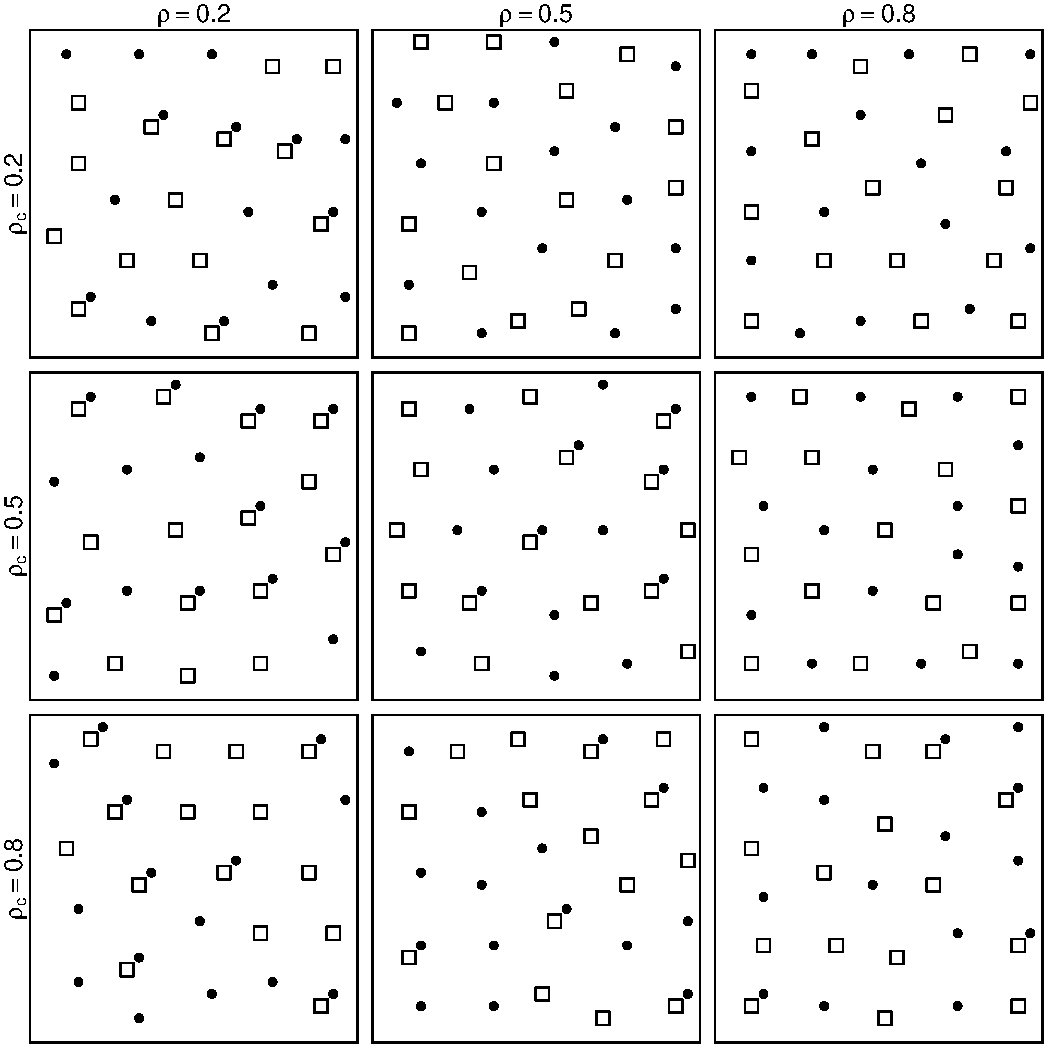
\includegraphics[width=0.5\textwidth]{saablup_NS3.pdf}
        \caption{Locally ostensibly MPEV-optimal designs for the NS4 large example.}\label{fig:mpevtoy}
        \end{center}
        \end{figure}

        \begin{figure}
        \begin{center}
        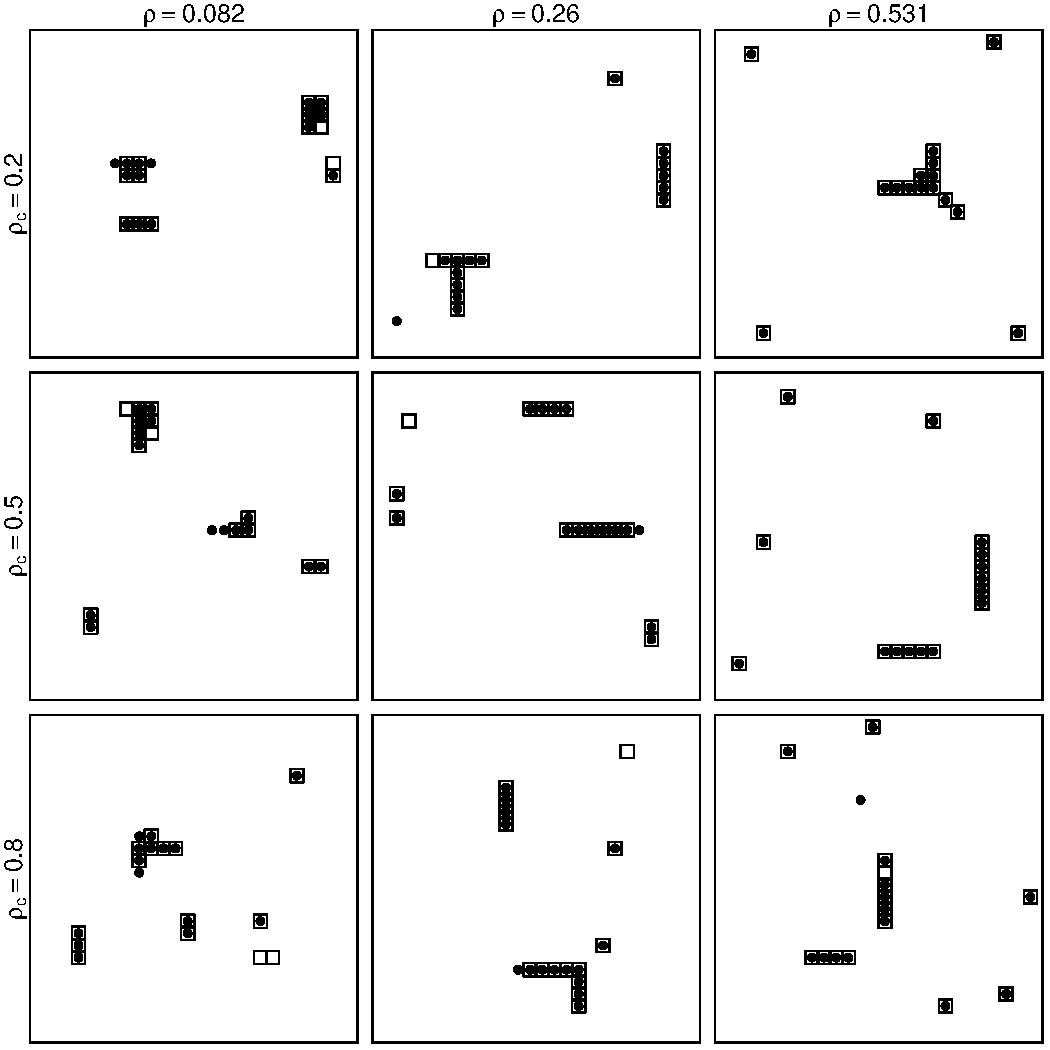
\includegraphics[width=0.5\textwidth]{saacovest_matern2.pdf}
        \caption{Locally ostensibly CPE-optimal designs for the Mat(1.5) large example.}\label{fig:mpevlarger}
        \end{center}
        \end{figure}


        \begin{figure}
        \begin{center}
        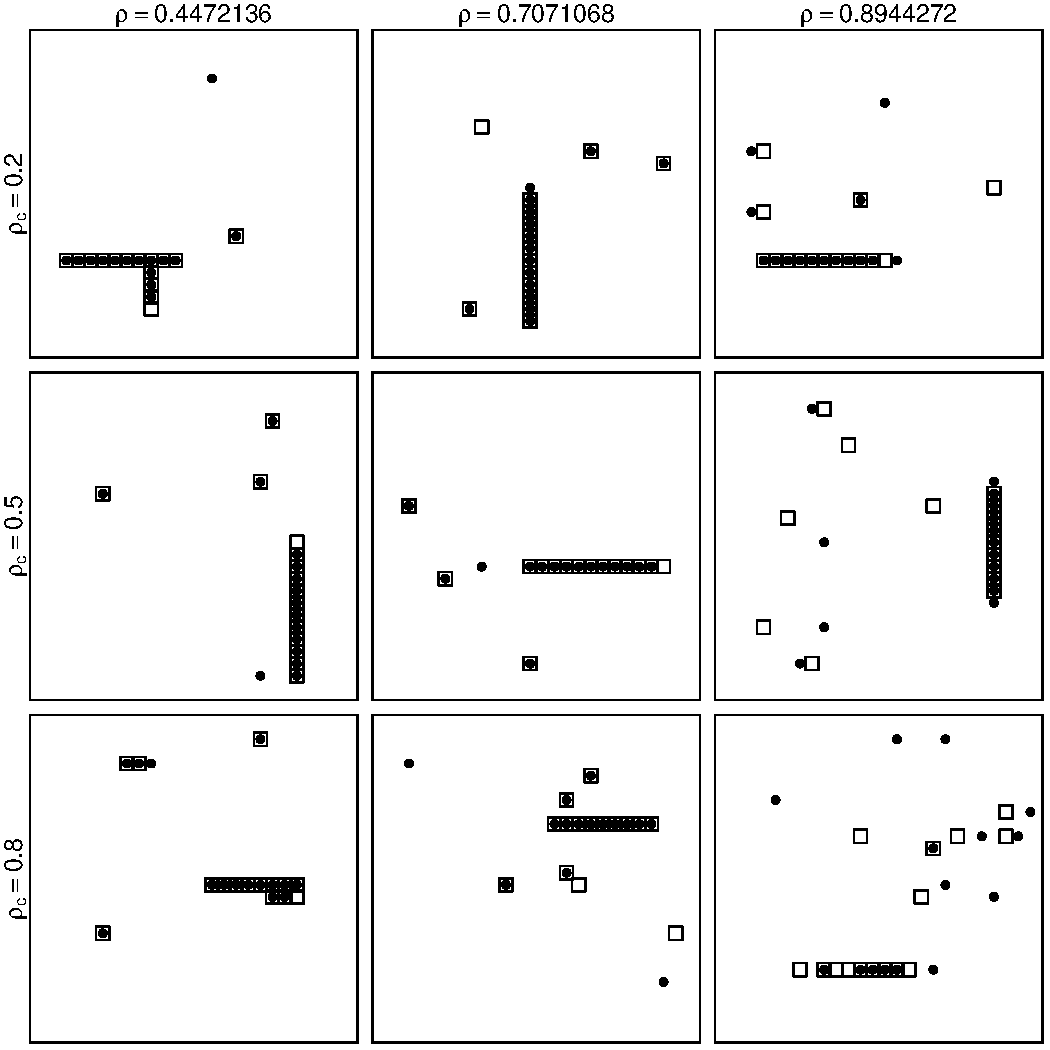
\includegraphics[width=0.5\textwidth]{saacovest_matern1.pdf}
        \caption{Locally ostensibly CPE-optimal designs for the Mat($\infty$) large example.}\label{fig:mpevlarger}
        \end{center}
        \end{figure}

        \begin{figure}
        \begin{center}
        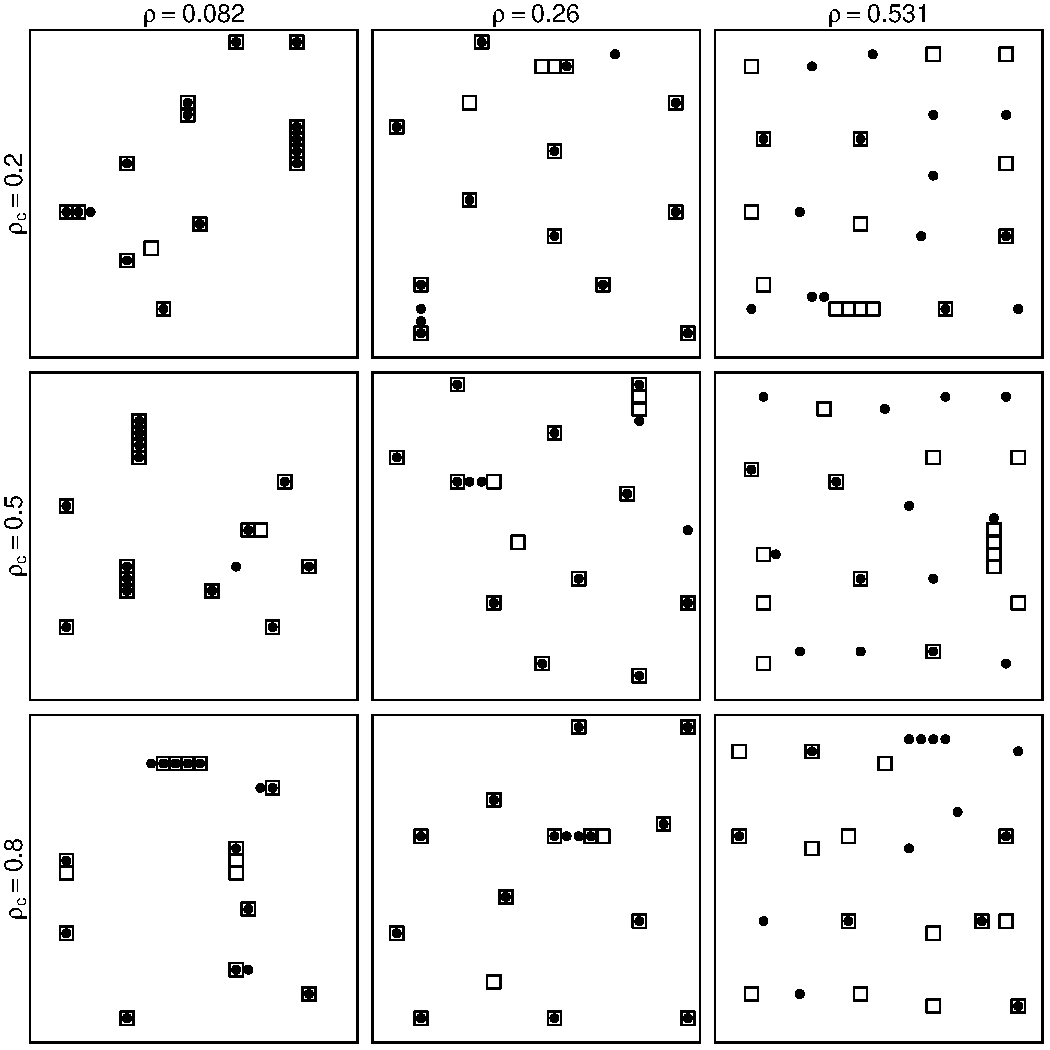
\includegraphics[width=0.5\textwidth]{saaeblup_matern2.pdf}
        \caption{Locally ostensibly MEPEV-optimal designs for the Mat(1.5) large example.}\label{fig:mepevlarger}
        \end{center}
        \end{figure}

        \begin{figure}
        \begin{center}
        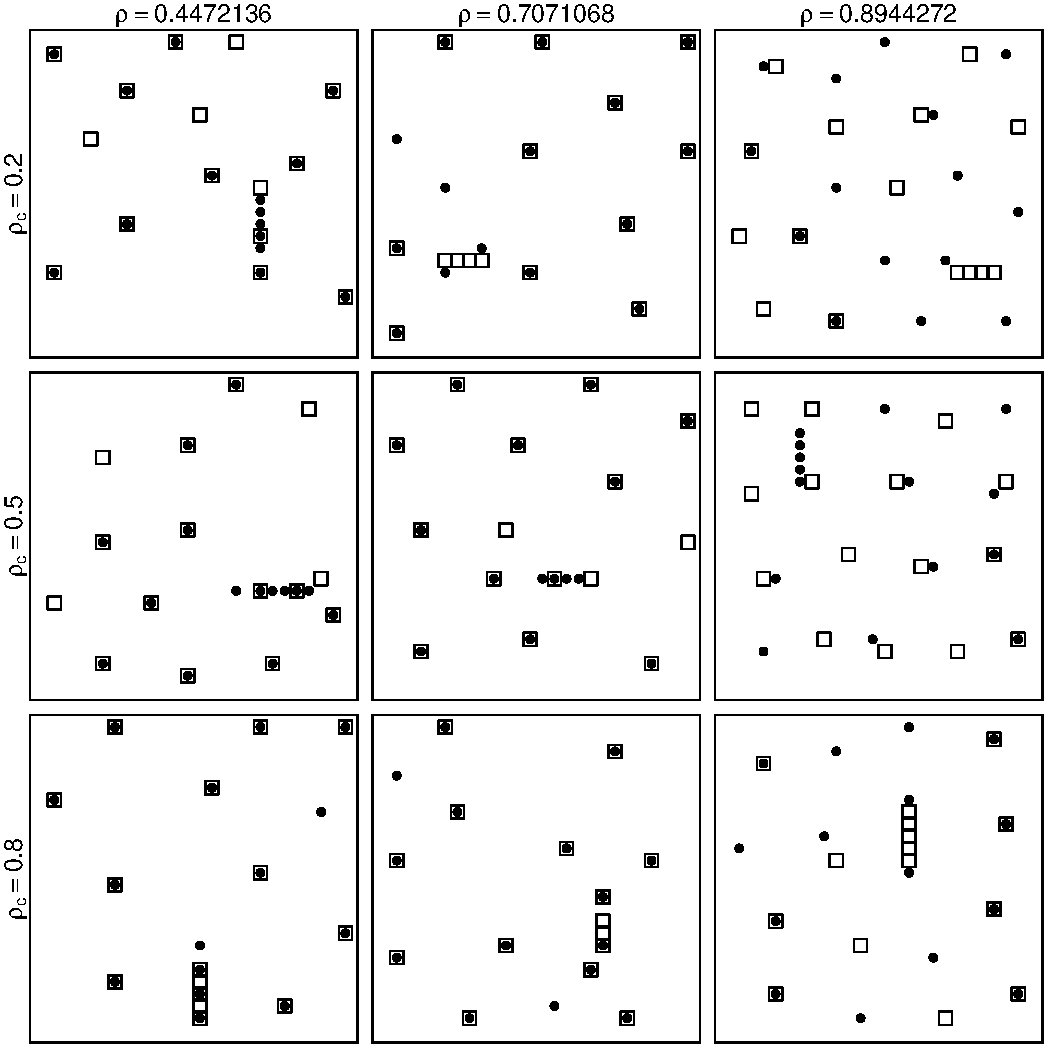
\includegraphics[width=0.5\textwidth]{saaeblup_matern1.pdf}
        \caption{Locally ostensibly MEPEV-optimal designs for the Mat($\infty$) large example.}\label{fig:mepevlarger}
        \end{center}
        \end{figure}

        \begin{figure}
        \begin{center}
        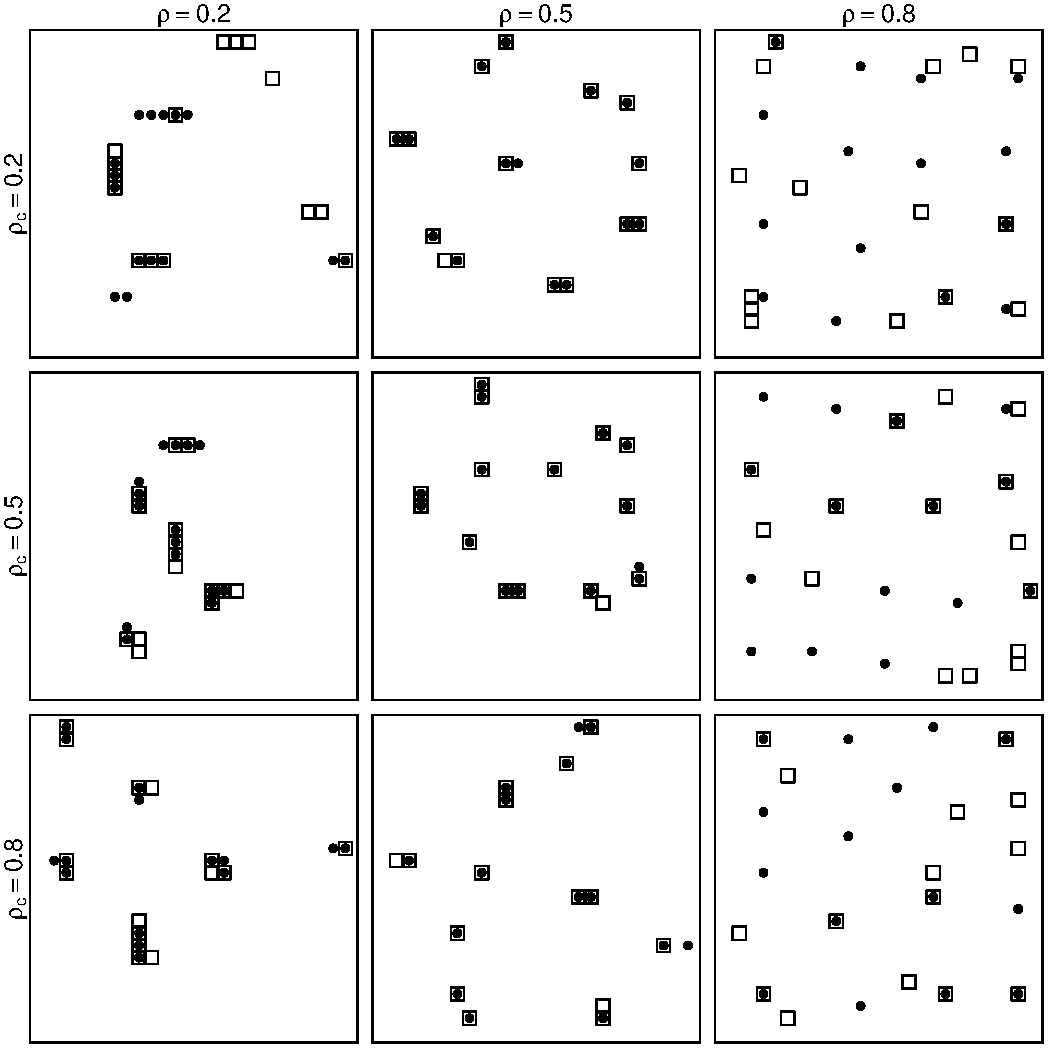
\includegraphics[width=0.5\textwidth]{saaeblup_NS2.pdf}
        \caption{Locally ostensibly MEPEV-optimal designs for the NS1 large example.}\label{fig:mepevlarger}
        \end{center}
        \end{figure}

        \begin{figure}
        \begin{center}
        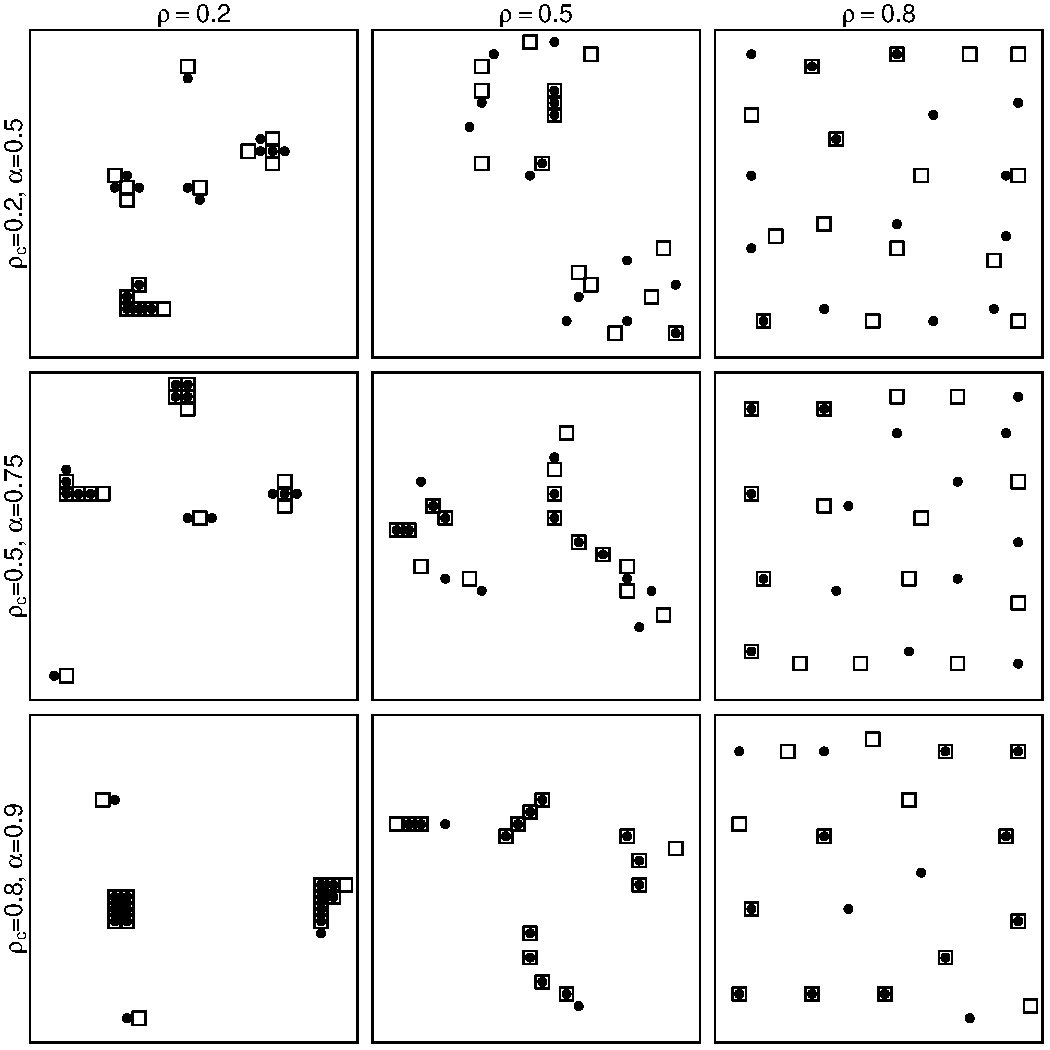
\includegraphics[width=0.5\textwidth]{saaeblup_NS1.pdf}
        \caption{Locally ostensibly MEPEV-optimal designs for the NS2 large example.}\label{fig:mepevlarger}
        \end{center}
        \end{figure}

        \begin{figure}
        \begin{center}
        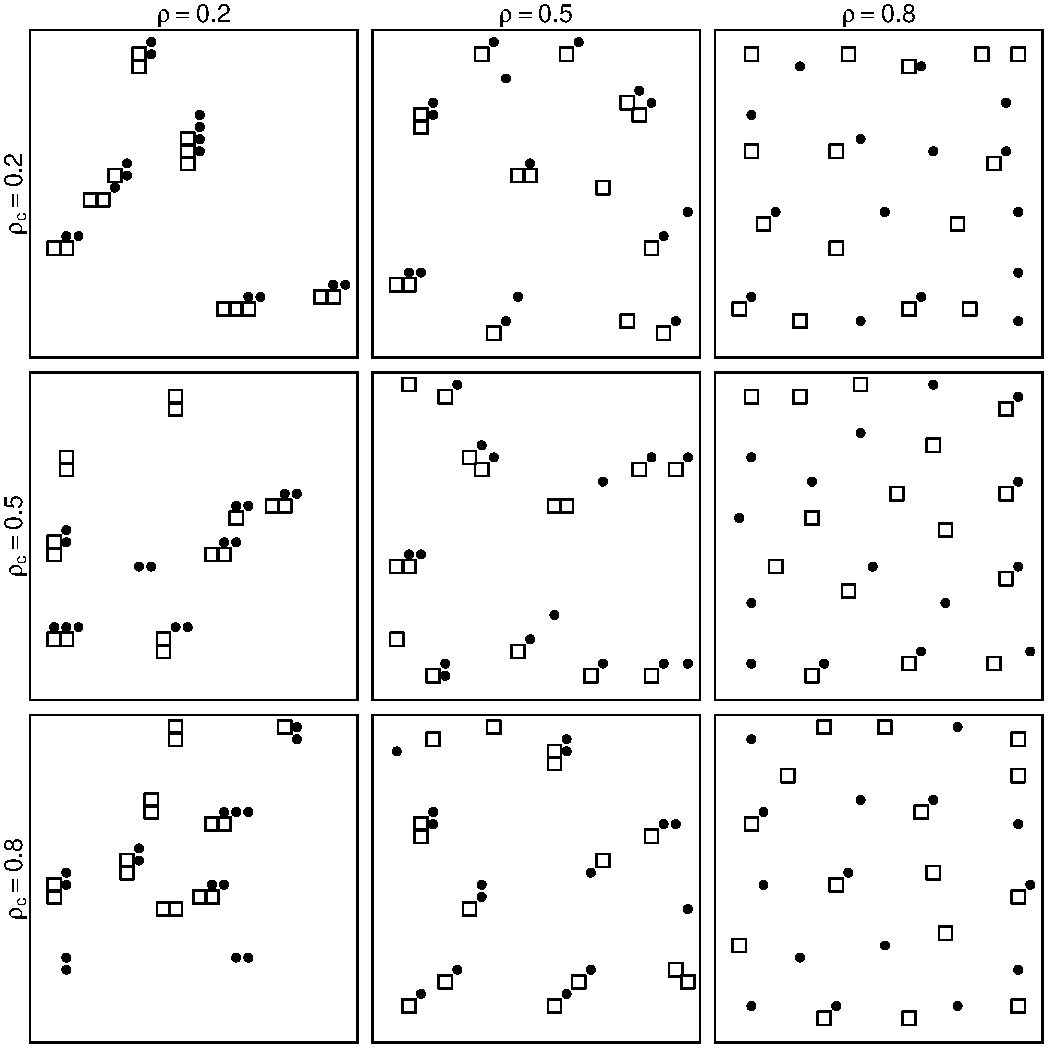
\includegraphics[width=0.5\textwidth]{saaeblup_NS3.pdf}
        \caption{Locally ostensibly MEPEV-optimal designs for the NS4 large example.}\label{fig:mepevlarger}
        \end{center}
        \end{figure}

        \begin{figure}
        \begin{center}
        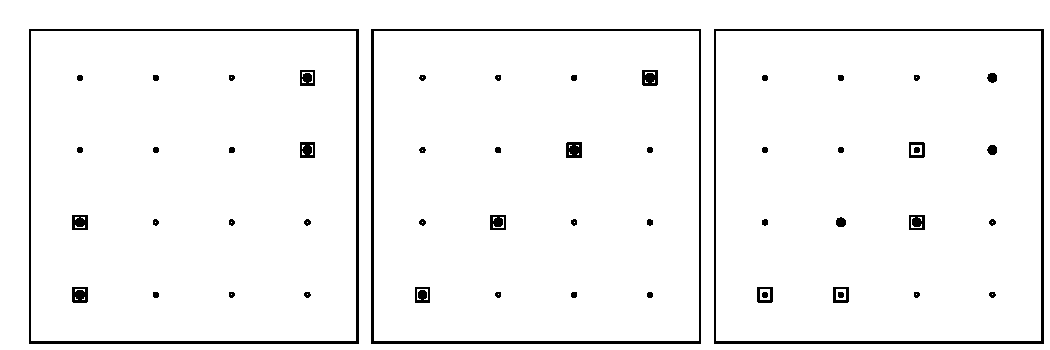
\includegraphics[width=0.5\textwidth]{covestns4toy.pdf}
        \caption{The superposition of CPE-optimal univariate designs, the CPE-optimal collocated design, and the CPE-optimal design (left to right) for the NS4 toy example when $\rho_c=\rho=0.2$.}\label{fig:cpens4toy}
        \end{center}
        \end{figure}

        \begin{figure}
        \begin{center}
        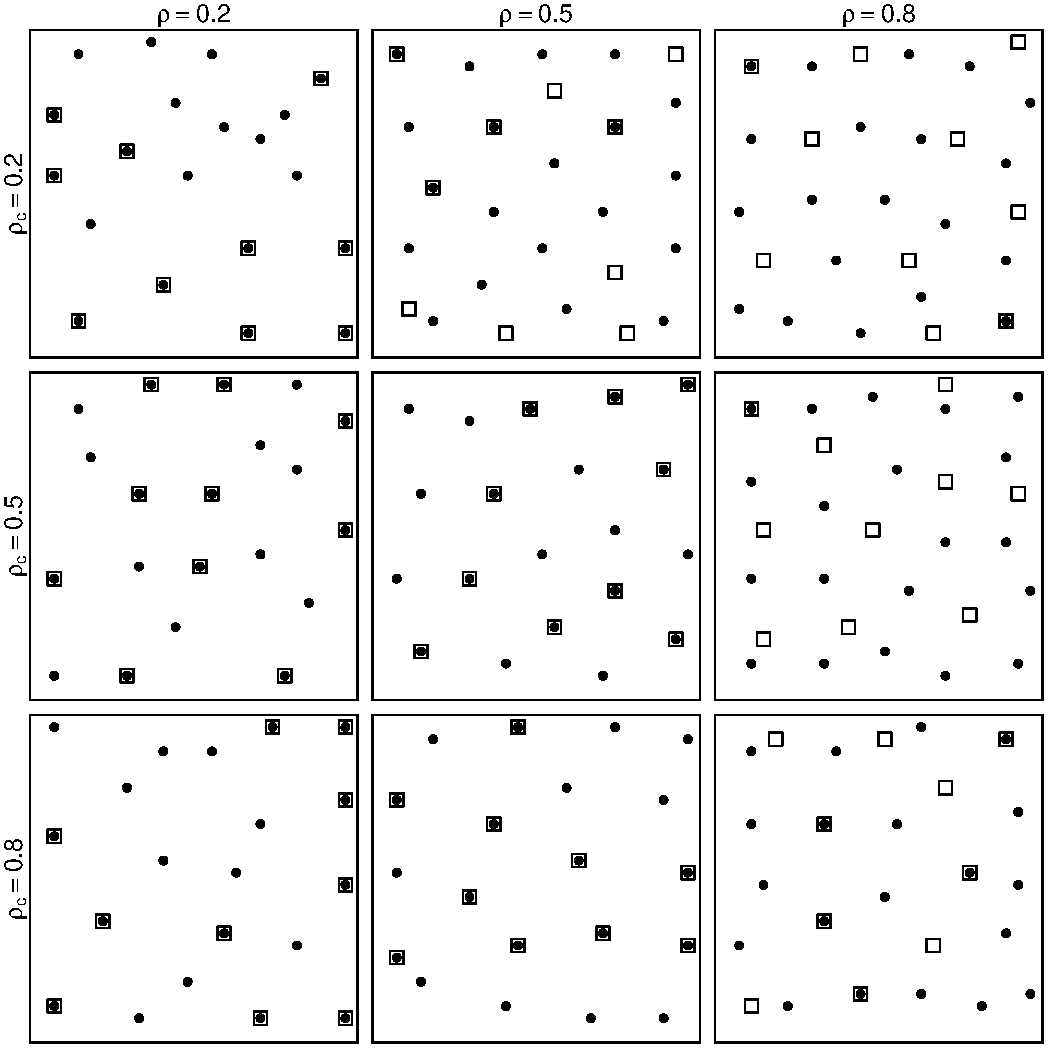
\includegraphics[width=0.5\textwidth]{saablup_NS2_imbalanced.pdf}
        \caption{Locally ostensibly MPEV-optimal unbalanced designs ($n_1=20,n_2=10$) for the NS2 large example.}
        \end{center}
        \end{figure}

        \begin{figure}
        \begin{center}
        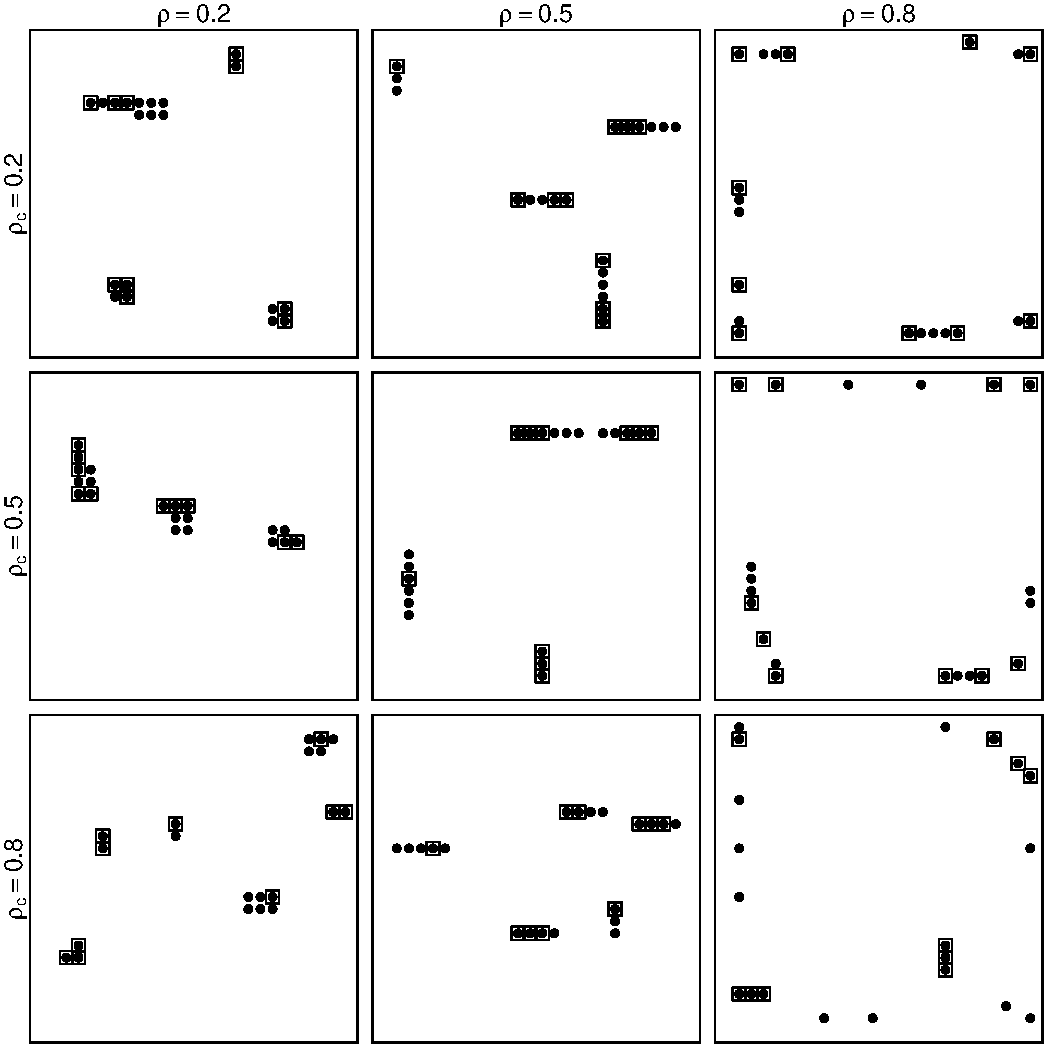
\includegraphics[width=0.5\textwidth]{saacovest_NS2_imbalanced.pdf}
        \caption{Locally ostensibly CPE-optimal unbalanced designs ($n_1=20,n_2=10$) for the NS2 large example.}
        \end{center}
        \end{figure}

        \begin{figure}
        \begin{center}
        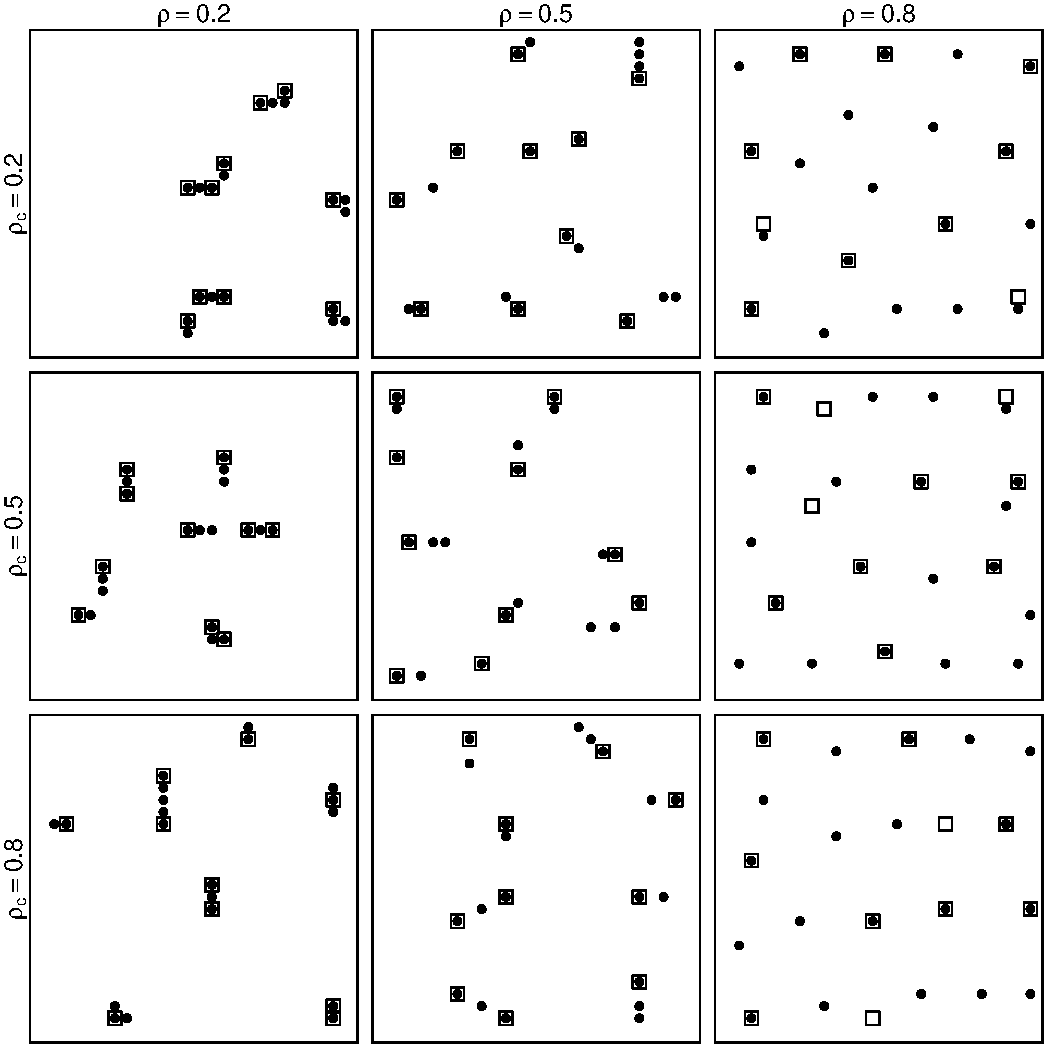
\includegraphics[width=0.5\textwidth]{saaeblup_NS2_imbalanced.pdf}
        \caption{Locally ostensibly MEPEV-optimal unbalanced designs ($n_1=20,n_2=10$) for the NS2 large example.}
        \end{center}
        \end{figure}

        \begin{figure}
        \begin{center}
        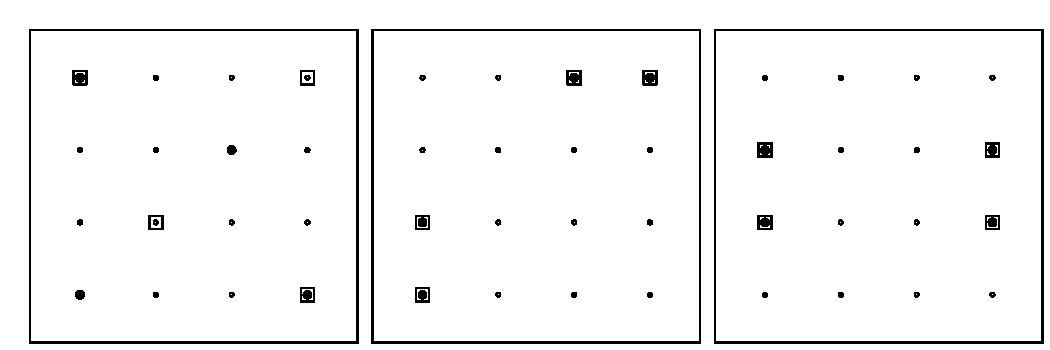
\includegraphics[width=0.5\textwidth]{desirability.pdf}
        \caption{Locally MPEV-, CPE-, and MEPEV-optimal compromise designs (left to right), using a desirability function, for the Mat(0.5) toy example.}
        \end{center}
        \end{figure}

        \begin{figure}
        \begin{center}
        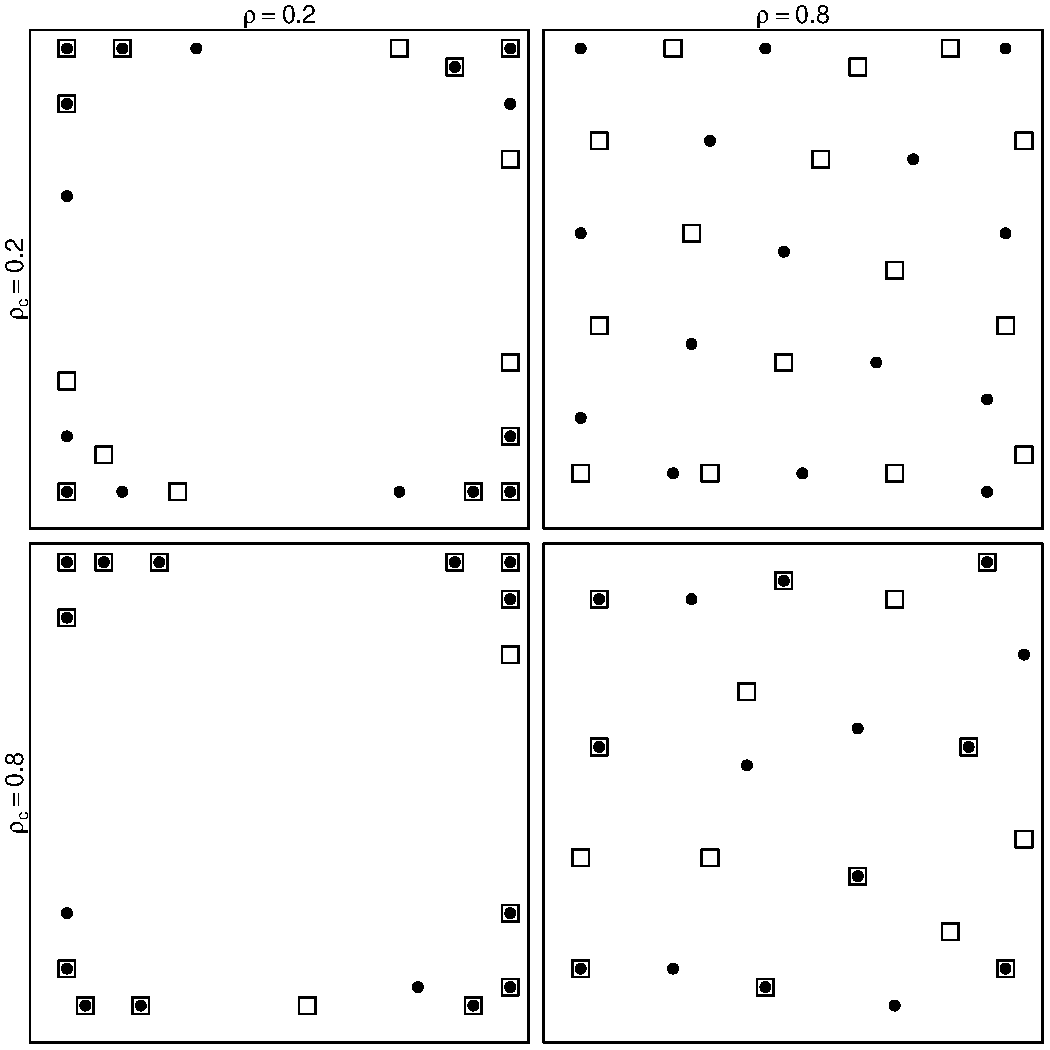
\includegraphics[width=0.33\textwidth]{saablup_planar.pdf}
        \caption{Locally ostensibly MPEV-optimal designs for the Mat(0.5) large example with planar mean.}\label{fig:mepevlarger}
        \end{center}
        \end{figure}

\newpage

\section{Simulated Annealing Algorithm}
\normalsize
%\vspace{.05in}
%\newline

For general use, we propose the following simulated
        annealing algorithm (SAA) to search for the locally optimal design for a fixed vector $\btheta$ of covariance parameters. The algorithm consists of the following steps:

        \begin{itemize}
            \item[1.] Randomly choose a design $D_{0}$,
            then compute $\gamma(D_{0};\btheta)$, where $\gamma(\cdot)$ is the
            corresponding criterion function that we wish to
            minimize. Set the initial values for the ``cooling
            factor''
            and ``distance factor'', $\tau_{0}$ and $h_{max_{0}}$,
            respectively.
            \item[2.] Randomly select a point in $D_{0}$ and move it $h$ units in a randomly selected direction,
            where $h$ has a uniform distribution on $[0,h_{max_{0}}]$.  If the move takes the point
            to a location outside the design region, then the point is returned to
            its original location and a new move is generated at
            random until the moved point falls into the design region. Call this new design $D_{1}$.
            \item[3.] Calculate $\gamma(D_{1};\btheta)$. Then the transition
            $D_{0} \rightarrow D_{1}$ is accepted with the following
            probability:
                $$P_{\tau}(D_{0}\rightarrow D_{1})=\left\{
                    \begin{array}{ll}
                        1, & \hbox{if $\gamma(D_{1};\btheta)\leq \gamma(D_{0};\btheta)$;} \\
                        \exp\{[\gamma(D_{0};\btheta)-\gamma(D_{1};\btheta)]/\tau_{0}\}, & \hbox{if $\gamma(D_{1};\btheta)> \gamma(D_{0};\btheta)$.}
                    \end{array}
                    \right.$$

            \item[4.] Repeat steps 2-3 for $N_{sim}$ (sufficiently large)
            times.
            \item[5.] At the end of the $N_{sim}$ repetitions, reduce
            the ``cooling factor'' and ``distance factor'' to
            $\tau_{k+1}=\alpha_{\tau}\tau_{k}$, $h_{max_{k+1}}=\alpha_{h}h_{max_{k}}$.
            \item[6.] Repeat steps 2-5 for $N_{t}$ times.
        \end{itemize}

        In this algorithm, $\tau_{0}$ was set so that $95\%$ or more
        of the moves would be accepted before the first cooling step;
        $\alpha_{\tau}$ was set so that the acceptance rate would be below $0.1\%$
        on the final step; $h_{max_{0}}$ was set
        at half the length of the region to be sampled; and $\alpha_{h}$ was set such
        that the final $h_{max}$ was 0.5 unit.

        For our featured examples, the set of candidate design points is a finite rectangular grid
so we can only move a point in four directions: north, south,
east and west.  Also, the distance
to be moved is generated from a discrete uniform distribution, i.e.,
the distance must be an integer multiple of the unit spacing. In
all cases, we chose $N_{sim}=1000$ and $N_{t}=1000$.

        In our larger example, it took a few hours for the algorithm to
        converge to a (local) minimum, given a specific set of
        values for $\rho_c$ and $\rho$.
Different starting designs were used, including regular square grid, random, and clustered
designs, each in completely collocated, completely disjoint, and mixed forms.
Regardless of the design criterion, the starting design had no discernible effect on the qualitative
characteristics and very little effect on either the criterion value of the final design or the number of
iterations required to achieve convergence.  Thus, the results are extremely robust to the choice of starting design.

As a check, we applied the SAA to the toy examples.  In every case, the SAA converged to the same locally optimal design (or one within the same equivalence class) obtained by complete enumeration.  However, in some cases it took longer to find this design using the SAA than by complete enumeration. A potential improvement of the SAA is to adaptively restrict the allowable directions a point may be moved, so as to eliminate the need to discard beyond-the-boundary moves from points on or near the boundary.

\newpage
%\noindent \Large{\textbf{Appendix B: Proof of Theorem 1}}\par
\section{Proof of Theorem 1}
\normalsize
%\vspace{.05in}
%\newline

\noindent \textbf{Proof of (a):}\par
Without loss of generality assume $m=2$.  Since the cross-correlation is zero,
\[ \bSigma_{00}=\left(\begin{array}{cc}
\sigma_1^2 & 0 \\
0 & \sigma_{2}^2 \end{array} \right),\quad\quad
{\bf C}_0=\left(\begin{array}{cc}
\sigma_1^2{\bf c}_1 & {\bf 0} \\
{\bf 0} & \sigma_{2}^2{\bf c}_2 \end{array} \right),\quad\quad
\mbox{and}\quad\bSigma=\left(\begin{array}{cc}
\sigma_1^2{\bf R}_{11} & {\bf 0} \\
{\bf 0} & \sigma_{2}^2{\bf R}_{22} \end{array} \right)
\]
for certain vectors ${\bf c}_1$ and ${\bf c}_2$ and correlation matrices ${\bf R}_{11}$ and ${\bf R}_{22}$.
Substitution into (2) then establishes that the off-diagonal elements of ${\bf V}({\bf s}_0,\btheta,D)$ are zero, so that $|{\bf V}({\bf s}_0,\btheta,D)|$ is the product of its main diagonal elements, which are nonnegative.  Now recall the well-known fact that the best linear unbiased predictor of a variable at a site at which it is observed is merely the observed value of the variable at that site.  Thus if ${\bf s}_0\in D$, then at least one of the main diagonal elements of ${\bf V}({\bf s}_0,\btheta,D)$ is zero and thus $|{\bf V}({\bf s}_0,\btheta,D)|=0$.  For ${\bf s}_0\notin D$, $|{\bf V}({\bf s}_0,\btheta,D)|>0$.  The maximum of $|{\bf V}({\bf s},\btheta,D)|$ over all ${\bf s}\in{\cal P}$ therefore is minimized by making $D\cap{\cal P}$ as large as possible, i.e.\ by imposing no collocation whatsoever.  This completes the proof of part (a).
\vspace{.2in}
\newline
\noindent\textbf{Proof of (b):}\\
Again assume $m=2$ without loss of generality.  Consider first the value of $|{\bf V}|$ when the design is completely collocated, in which case $\bSigma=\bSigma_{00}\otimes{\bf I}_n$.  If ${\bf s}_0\in D$, then ${\bf C}_0=\bSigma_{00}\otimes{\bf e}_i$ for some $i=1,\ldots,n$, where ${\bf e}_i$ is the $n\times 1$ vector with 1 as its $i$th element and zeros elsewhere,
and
\begin{eqnarray*}
{\bf V}({\bf s}_0,\btheta,D) & = & \bSigma_{00}-(\bSigma_{00}\otimes{\bf e}_i)^{'}(\bSigma_{00}\otimes{\bf I}_n)^{-1}(\bSigma_{00}
\otimes{\bf e}_i)+[{\bf I}_2-({\bf I}_2\otimes {\bf 1}_n)^{'}(\bSigma_{00}\otimes{\bf I}_n)^{-1}(\bSigma_{00}
\otimes{\bf e}_i)]^{'} \\
& & \times [({\bf I}_2\otimes{\bf 1}_n)^{'}(\bSigma_{00}\otimes{\bf I}_n)^{-1}({\bf I}_2\otimes {\bf 1}_n)]^{-1}[{\bf I}_2-({\bf I}_2\otimes {\bf 1}_n)^{'}(\bSigma_{00}\otimes{\bf I}_n)^{-1}(\bSigma_{00}
\otimes{\bf e}_i)] \\
& = & {\bf 0}.
\end{eqnarray*}
If, on the other hand, ${\bf s}_0\notin D$, then ${\bf C}_0={\bf 0}$ and
\begin{eqnarray*}
{\bf V}({\bf s}_0,\btheta,D) & = & \bSigma_{00}+{\bf I}_2^{\prime}[({\bf I}_2\otimes{\bf 1}_n)^{'}(\bSigma_{00}\otimes{\bf I}_n)^{-1}({\bf I}_2\otimes {\bf 1}_n)]^{-1}{\bf I}_2 \\
& = & \left(\frac{n+1}{n}\right)\bSigma_{00}.
\end{eqnarray*}
Thus when the design is completely collocated,
\begin{equation}\label{eq:detvcollocated}
\max_{{\bf s}\in{\cal P}}|{\bf V}({\bf s},\btheta,D)|=\sigma_1^2\sigma_2^2(1-\rho_c^2)\left(\frac{n+1}{n}\right)^2.
\end{equation}

If the design is not completely collocated, then, letting $n-n_0$ denote the number of collocated sites in the design, the sites can be ordered in such a way that
\[ \bSigma=\left(\begin{array}{cc}
\mbox{diag}(\sigma_1^2,\sigma_2^2)\otimes{\bf I}_{n_0} & {\bf 0} \\
{\bf 0} & \bSigma_{00}\otimes{\bf I}_{n-n_0} \end{array} \right)\quad\mbox{and}\quad
{\bf X}=\left(\begin{array}{c}
{\bf I}_2\otimes{\bf 1}_{n_0} \\
{\bf I}_2\otimes{\bf 1}_{n-n_0} \end{array} \right) .
\]
Furthermore, since card$({\cal P})>2n$ by assumption, there is at least one site ${\bf s}_0\in{\cal P}$ for which ${\bf s}_0\notin D$.  For such a site, ${\bf C}_0={\bf 0}$ and thus
${\bf V}({\bf s}_0,\btheta,D)=\bSigma_{00}+[n_0\mbox{diag}(1/\sigma_1^2,1/\sigma_2^2)+(n-n_0)\bSigma_{00}^{-1}]^{-1}$.
After some algebra, we obtain
\begin{equation}\label{eq:detv}
|{\bf V}({\bf s}_0,\btheta,D)|=\sigma_1^2\sigma_2^2(n^2-n_0^2\rho_c^2)^{-2}[(n^2+n-n_0^2\rho_c^2-n_0\rho_c^2)^2-\rho_c^2(n^2+n-n_0^2\rho_c^2-n_0)^2].
\end{equation}
After considerably more algebra and an appropriate factorization, it can be shown that the term in brackets in (\ref{eq:detv}) is equal to $(1-\rho_c^2)(n^2-n_0^2\rho_c^2)[(n+1)^2-n_0^2\rho_c^2]$.  Thus
\[ |{\bf V}({\bf s}_0,\btheta,D)|=\sigma_1^2\sigma_2^2(1-\rho_c^2)\left(\frac{(n+1)^2-n_0^2\rho_c^2}{n^2-n_0^2\rho_c^2}\right), \]
which, for $\rho_c\neq 0$, is strictly larger than (\ref{eq:detvcollocated}).  This completes the proof of part (b).

%\noindent \Large{\textbf{Appendix C: Proof of Theorem 2}}\par

\section{Proof of Theorem 2}
\normalsize
%\vspace{.05in}
%\newline

\noindent \textbf{Proof of (a):}\par
The distinct sites of a collocated design may be represented as ${\bf s}_1,{\bf s}_2,\ldots,{\bf s}_n$.  This, together with the specified conditions on the mean function, implies that ${\bf X}_1={\bf X}_2=\cdots={\bf X}_n$ and thus that ${\bf X}={\bf I}_m\otimes{\bf X}_1$.  Similarly, ${\bf X}_0={\bf I}_m\otimes[{\bf x}_1({\bf s}_0)]^{\prime}$.  Furthermore, the separability of the process yields $\bSigma=\bSigma_{00}\otimes{\bf R}$ and ${\bf C}_0=\bSigma_{00}\otimes{\bf r}_0$, where ${\bf R}$ is the $n\times n$ matrix of spatial correlations among the observations at ${\bf s}_1,\ldots,{\bf s}_n$ on any one of the $m$ variables and ${\bf r}_0$ is the $n\times 1$ vector of spatial correlations between the observations at ${\bf s}_1,\ldots,{\bf s}_n$ on any variable and that same variable at ${\bf s}_0$.  Then, using equation (2) of Section 3.1, the covariance matrix of prediction errors associated with the BLUP of ${\bf Z}({\bf s}_0)$ is
\begin{eqnarray*}
{\bf V}({\bf s}_{0},\btheta,D) & = & \bSigma_{00}-(\bSigma_{00}\otimes{\bf r}_0)^{\prime}
(\bSigma_{00}\otimes{\bf R})^{-1}(\bSigma_{00}\otimes{\bf r}_0) \\
& & +[({\bf I}_m\otimes[{\bf x}_1({\bf s}_0)]^{\prime})-({\bf I}_m\otimes{\bf X}_1)^{\prime}(\bSigma_{00}\otimes{\bf R})^{-1}(\bSigma_{00}\otimes{\bf r}_0)]^{\prime} \\
& & \times[({\bf I}_m\otimes{\bf X}_1)^{\prime}(\bSigma_{00}\otimes{\bf R})^{-1}({\bf I}_m\otimes{\bf X}_1)]^{-1} \\
& & \times[({\bf I}_m\otimes[{\bf x}_1({\bf s}_0)]^{\prime})-({\bf I}_m\otimes{\bf X}_1)^{\prime}(\bSigma_{00}\otimes{\bf R})^{-1}(\bSigma_{00}\otimes{\bf r}_0)] \\
& = & \bSigma_{00}\otimes[1-{\bf r}_0^{\prime}{\bf R}^{-1}{\bf r}_0+({\bf x}_1({\bf s}_0)-{\bf X}_1^{\prime}{\bf R}^{-1}{\bf r}_0)^{\prime}({\bf X}_1^{\prime}{\bf R}^{-1}{\bf X}_1)^{-1}({\bf x}_1({\bf s}_0)-{\bf X}_1^{\prime}{\bf R}^{-1}{\bf r}_0)] \\
& = & \bSigma_{00}\otimes[v_1({\bf s}_0,\btheta,D)/C_{11}({\bf s}_0,{\bf s}_0;\btheta)],
\end{eqnarray*}
where $v_1({\bf s}_0,\btheta,D)$ is the prediction error variance associated with the univariate BLUP of the first component of ${\bf Z}({\bf s}_0)$.  Thus
$|{\bf V}({\bf s}_0,\btheta,D)|=|\bSigma_{00}|\cdot\left[v_1({\bf s}_0,\btheta,D)/C_{11}({\bf s}_0,{\bf s}_0;\btheta)\right]^m$, so that the minimization of $\max_{{\bf s}\in{\cal P}}|{\bf V}({\bf s},\btheta,D)|$ over the design space is equivalent to the minimization of $\max_{{\bf s}\in{\cal P}}v_1({\bf s},\btheta,D)$.  This completes the proof of part (a).
\vspace{.2in}
\newline
\noindent\textbf{Proof of (b):}\\
As noted in the proof of part (a), $\bSigma=\bSigma_{00}\otimes{\bf R}$. Since $\bSigma_{00}$ is symmetric, we have that $\bSigma_{00}=\bOmega\mathbf{\Lambda}\bOmega'$, where $\mathbf{\Lambda}$ is a diagonal matrix whose positive elements $\lambda_{1},\ldots,\lambda_m$ are the eigenvalues of $\bSigma_{00}$ and
$\bOmega=(\omega_{ij})$ is the corresponding matrix of orthonormal eigenvectors.  Let $\blambda=(\lambda_1,\ldots,\lambda_m)'$, let $\bomega$ be the $m(m-1)/2\times 1$ vector of below-diagonal elements of $\bOmega$, let $\brho$ be the $s\times 1$ vector of spatial correlation parameters, and let
$\mb{\xi}=(\xi_{i})=(\blambda',\bomega',\brho')'$.  For the REML information matrix ${\bf I}(\btheta,D)$, we have ${\bf I}(\btheta,D)={\bf JI}(\bxi,D){\bf J}^{'}$ where ${\bf J}=\partial\bxi/\partial\btheta$ is not affected by the design.  Thus the CPE-optimal design is that which minimizes $1/|{\bf I}(\bxi,D)|$.  The $(i,j)$th element of ${\bf I}(\mb{\xi},D)$ is given by $\frac{1}{2}\text{tr}(\mathbf{P}\frac{\partial\mathbf{\Sigma}}{\partial\xi_{i}}\mathbf{P}\frac{\partial\mathbf{\Sigma}}{\partial\xi_{j}})$, where $\mathbf{P=(\bOmega
\mathbf{\Lambda}^{-1}\bOmega')\otimes P}_{u}$, $\mathbf{P}_{u}={\bf R}^{-1}-{\bf R}^{-1}{\bf X}_{1}({\bf X}^{'}_{1}{\bf R}^{-1}{\bf X}_{1})^{-1}{\bf X}^{'}_{1}{\bf R}^{-1}$, and
\[ \frac{\partial \mathbf{\Sigma}}{\partial \xi_{i}}=\left\{\begin{array}{ll}
\bOmega\frac{\partial\mathbf{\Lambda}}{\partial\xi_{i}}\bOmega'\otimes {\bf R}, & i=1,\ldots,m; \\
\left(\frac{\partial\bOmega}{\partial\xi_{i}}\mathbf{\Lambda}\bOmega'+
  \bOmega\mathbf{\Lambda}\frac{\partial\bOmega'}{\partial\xi_{i}}\right)\otimes {\bf R}, & i=m+1,\ldots,\frac{m(m+1)}{2}; \\
(\bOmega\mathbf{\Lambda}\bOmega')\otimes\frac{\partial {\bf R}}{\partial\xi_{i}}, & i=\frac{m(m+1)}{2}+1,\ldots,\frac{m(m+1)}{2}+s. \end{array} \right.
\]
When $i=1,\ldots,m$ and $j=1,\ldots,m$, we have that
\[ \frac{1}{2}\text{tr}(\mathbf{P}\frac{\partial\mathbf{\Sigma}}{\partial\xi_{i}}\mathbf{P}\frac{\partial\mathbf{\Sigma}}{\partial\xi_{j}})
   = \frac{1}{2}\text{tr}\left(\mathbf{\Lambda}^{-1}\frac{\partial\mathbf{\Lambda}}{\partial\xi_{i}}
   \mathbf{\Lambda}^{-1}\frac{\partial\mathbf{\Lambda}}{\partial\xi_{j}}\right)\text{tr}\left( {\bf P}_u{\bf R}{\bf P}_u{\bf R} \right)
  =\left\{
     \begin{array}{ll}
       0, & \hbox{$i\neq j$;} \\
       \frac{n-p}{2\lambda_{i}^2}, & \hbox{$i=j$.}
     \end{array}
   \right.
\]
When $i=1,\ldots,m$ and $j=m+1,\ldots,\frac{m(m+1)}{2}$, we have that
\[ \frac{1}{2}\text{tr}(\mathbf{P}\frac{\partial\mathbf{\Sigma}}{\partial\xi_{i}}\mathbf{P}\frac{\partial\mathbf{\Sigma}}{\partial\xi_{j}})
    = \frac{n-p}{2}\left[\text{tr}\left(\frac{\partial\mathbf{\Lambda}}{\partial\xi_{i}}\mathbf{\Lambda^{-1}}
    \left\{\bOmega'\frac{\partial\bOmega}{\partial\xi_{j}}+\frac{\partial\bOmega'}{\partial\xi_{j}}\bOmega\right\}\right)\right]=0
\]
since $\bOmega'\frac{\partial\bOmega}{\partial\xi_{j}}+\frac{\partial\bOmega'}{\partial\xi_{j}}\bOmega
  =\frac{\partial(\bOmega'\bOmega)}{\partial\xi_j}=\frac{\partial \mathbf{I}}{\partial\xi_{j}}=0$.
Similar calculations yield
\[ \frac{1}{2}\text{tr}(\mathbf{P}\frac{\partial\mathbf{\Sigma}}{\partial\xi_{i}}\mathbf{P}\frac{\partial\mathbf{\Sigma}}{\partial\xi_{j}})
     = \left\{ \begin{array}{ll} \frac{1}{2\lambda_{i}}\text{tr}\left({\bf P}_u\frac{\partial
     \mathbf{R}}{\partial\xi_{j}}\right) & i=1,\ldots,m; \, j=\frac{m(m+1)}{2}+1,\ldots,\frac{m(m+1)}{2}+s \\
\frac{n-p}{2}k_{ij} & i,j=m+1,\ldots,\frac{m(m+1)}{2} \\
0 & i=m+1,\ldots,\frac{m(m+1)}{2}; \, j=\frac{m(m+1)}{2}+1,\ldots,\frac{m(m+1)}{2}+s \\
\frac{m}{2}\text{tr}\left(\mathbf{P}_{u}\frac{\partial
\mathbf{R}}{\partial\xi_{i}}\mathbf{P}_{u}\frac{\partial
\mathbf{R}}{\partial\xi_{j}}\right) & i,j=\frac{m(m+1)}{2}+1,\ldots,\frac{m(m+1)}{2}+s
\end{array}\right.
\]
where $k_{ij}=\text{tr}\left[\bOmega\mathbf{\Lambda^{-1}}\bOmega'\left(\frac{\partial\bOmega}{\partial\xi_{i}}\mathbf{\Lambda}\bOmega'+
  \bOmega\mathbf{\Lambda}\frac{\partial\bOmega'}{\partial\xi_{i}}\right)\bOmega\mathbf{\Lambda^{-1}}\bOmega'\left(\frac{\partial\bOmega}{\partial\xi_{j}}\mathbf{\Lambda}\bOmega'+
  \bOmega\mathbf{\Lambda}\frac{\partial\bOmega'}{\partial\xi_{j}}\right)\right]$ and we have used the identity ${\bf P}_u{\bf RP}_u={\bf P}_u$.

Hence
\[ \mathbf{I}(\mb\xi,D) = \left(
    \begin{array}{ccc}
      \mathbf{I}_{11}
       & \mathbf{0}
        &  \mathbf{I}_{13}
       \\
\mathbf{0} & \mathbf{I}_{22} & \mathbf{0}
          \\
\mathbf{I}_{13}^{'}
       & \mathbf{0}
        & \mathbf{I}_{33}\\
    \end{array}
  \right)
\]
where $\mathbf{I}_{11}$ is the $m\times m$ diagonal matrix whose $i$th diagonal element is $\frac{n-p}{2\lambda_{i}^2}$,
$\mathbf{I}_{13}$ is the $m\times s$ matrix whose $(i,j)$th element is given by $\frac{1}{2\lambda_{i}}\text{tr}\left({\bf P}_u\frac{\partial\mathbf{R}}{\partial\xi_{\frac{m(m+1)}{2}+j}}\right)$, $\mathbf{I}_{22}$ is the $\frac{m(m-1)}{2}\times \frac{m(m-1)}{2}$ matrix whose $(i,j)$th element is $\left(\frac{n-p}{2}\right)k_{ij}$, and $\mathbf{I}_{33}$ is the $s\times s$ matrix whose $(i,j)$th element is given by $\frac{m}{2}\text{tr}\left(\mathbf{P}_{u}\frac{\partial
\mathbf{R}}{\partial\xi_{\frac{m(m+1)}{2}+i}}\mathbf{P}_{u}\frac{\partial
\mathbf{R}}{\partial\xi_{\frac{m(m+1)}{2}+j}}\right)$.  Observe that $\mathbf{I}_{11}$ and $\mathbf{I}_{22}$ do not depend on the design $D$.
Thus we may write, using well-known results on determinants of partitioned matrices,
\[ |\mathbf{I}(\mb\xi,D)| = |\mathbf{I}_{11}||\mathbf{I}_{22}||\mathbf{I}_{33}-\mathbf{I}_{13}^{'}\mathbf{I}_{11}^{-1}\mathbf{I}_{13}|.
\]
It is easily verified that $\mathbf{I}_{13}^{'}\mathbf{I}_{11}^{-1}\mathbf{I}_{13}$ is an $s\times s$ matrix whose $(i,j)$th element is given by
\[ \frac{m}{2(n-p)}\text{tr}\left({\bf P}_u\frac{\partial\mathbf{R}}{\partial\xi_{\frac{m(m+1)}{2}+i}}\right)\text{tr}\left({\bf P}_u\frac{\partial\mathbf{R}}{\partial\xi_{\frac{m(m+1)}{2}+j}}\right).
\]
Hence, $$|\mathbf{I}(\mb\xi,D)|=\left(\frac{2m\sigma_{1}^4}{n-p}\right)|\mathbf{I}_{11}||\mathbf{I}_{22}||\mathbf{I}_{u}(\sigma_{1}^2,\brho,D)|,$$
where $\mathbf{I}_{u}(\sigma_{1}^2,\brho,D)$ is the REML information matrix for the corresponding univariate design problem. It follows that minimizing $1/|{\bf I}(\bxi,D)|$ with respect to $D$ is equivalent to minimizing its univariate counterpart $1/|{\bf I}_{u}(\sigma_{1}^2,\brho,D)|$.
This completes the proof of part (b).

\end{document}
%%%%%%%%%%%%%%%%%%%%%%%%%%%%%%%%%%%%%%%%%%%%%%%%%%%%%%%%%%%%%%%%%%%%%%%%%%%%%%%%%%%%%%%%%%%%%%%%%%%%%%%%%%%%%%%%%
